\documentclass[11pt]{article}
\usepackage[utf8]{inputenc}
\usepackage[margin=1in]{geometry}
\usepackage{natbib}
\bibliographystyle{abbrvnat}
\usepackage{amsmath}
\usepackage{amssymb}
\usepackage{comment}
\usepackage{amsthm}
\geometry{a4paper}
\usepackage{graphicx}
\usepackage{booktabs}
\usepackage{array}
\usepackage{paralist}
\usepackage{verbatim}
\usepackage{subfig}
\usepackage{multirow}
\usepackage{wrapfig}
\usepackage{rotating}
\usepackage{fancyhdr}
\usepackage{hyperref}
\pagestyle{fancy}
\renewcommand{\headrulewidth}{0pt}
\lhead{}\chead{}\rhead{}
\lfoot{}\cfoot{\thepage}\rfoot{}
\usepackage{sectsty}
\allsectionsfont{\sffamily\mdseries\upshape}
\usepackage{algorithm}
\usepackage{algpseudocode}
\usepackage{fancyvrb}
\usepackage{parskip}
\usepackage{enumitem}
\usepackage{makecell}
\setlist{noitemsep} 
\setlength\parindent{0pt}

\title{Data Science - Assessed Coursework 2 \\ \small Statistical Analysis Report on Iranian Churn Dataset}
\author{CID: 01891103}
\date{}
\begin{document}
\maketitle

\section*{Abstract}

This report investigates customer churn patterns within an Iranian telecom dataset available on the UCI machine learning repository. The main aim is to model and predict the reasons for customer churning behaviour using various binary classification methodologies. A detailed exploratory data analysis (EDA) identified several skewed variables across varying scales and high correlations between covariates. Consequently, a square root transformation and standardisation are conducted before the modelling procedure. In this report, we implemented and compared the performance of the Stepwise Selected models (AIC \& BIC), Grouped LASSO (\texttt{gglasso}) and Support Vector Machine (SVM) models. The SVM model gives the best AUC while the BIC model predicts to gives the best accuracy on the test set. Further suggestions and concerns are provided at the end of this report. 



\section{Introduction}

The Iranian Telecom Company concerns a long-standing issue of managing customer churning, i.e. switching to other telecom providers. To better maintain customer loyalty and implement effective customer retention strategies, it would be crucial to know why customers churn and predict who will possibly churn based on the data collected by the company from the customers. 

Therefore, to help the Iranian telecom company to better predict customer behaviour hence increasing their profit, this report gives a detailed analysis of the churning behaviour dataset. The data is provided and maintained by \href{https://link.springer.com/article/10.1007/s00521-020-04850-6}{(Jafari-Marandi 2020)} and is open-source available on the \href{https://archive.ics.uci.edu/dataset/563/iranian+churn+dataset}{UCI machine learning repository}. 

  
\section{Exploratory Data Anlaysis}\label{sec:EDA}

The dataset contains 3150 observations (customers) with 14 columns, with no missing values in any cell. The columns consist of 1 column for the outcome binary indicator on the churning behaviour of the customers, 1 column indicating the Customer Value which is not an attribute to the modelling process according to (Jafari-Marandi 2020), and 12 feature/attribute columns describing the customer information including. The attributes are summarised in the Table \ref{table:features}

\begin{table}[h]
    \centering
    \begin{tabular}{@{}lll@{}}
    \toprule
    \textbf{Variable Name} & \textbf{Type} & \textbf{Description} \\ 
    \midrule
    Call Failure & continuous numeric & number of call failures \\
    Complains & binary & 0 = No complaint, 1 = Complaint \\
    Subscription Length & continuous numeric & total months of subscription \\
    Charge Amount & ordinal numeric & 0 lowest amount, 9 highest amount \\
    Seconds of Use & continuous numeric & total seconds of calls \\
    Frequency of use & continuous numeric & total number of calls \\
    Frequency of SMS & continuous numeric & total number of text messages \\
    Distinct Called Numbers & continuous numeric & total number of distinct phone calls \\
    Age Group & ordinal attribute & <15, 15-30, 30-45, 45-60, 60-75 \\
    Tariff Plan & binary & 1 = Pay as you go, 2 = contractual \\
    Status & binary & 1 = active, 2= non-active \\
    Churn & binary Class label & 1 = churn, 0 = non-churn \\
    \bottomrule
    \end{tabular}
    \caption{Summary of Outcome and Feature variables in the Dataset}
    \label{table:features}
\end{table}

Our dataset is split into 80-20 train-test split subsets, during the Exploratory Data Analysis (abbreviated as EDA later) sections, the \textbf{whole} dataset is analysed to detect the full patterns and provide a comprehensive overview of the dataset. Later in the modelling section, only the \textbf{training} set is used to select hyperparameters and train the models, where the \textbf{test} set is used only for examining the performance of the trained model and to compare their performance. 

\subsection{Univariate Analysis - distributions of variables}

From the univariate analysis plots, we notice that most continuous variables have high positive skewness, except the subscription length. This indicates that we may need to investigate further on the empirical logit plot later to decide if a transformation or scaling is needed. 

Also, the distribution of the continuous variables has very different scales, e.g., from 0-40 (call failures) to 0-20000 (Seconds of Use). This requires attention and consideration of standardization procedure before implementing some models which are sensitive to scales such as LASSO models. 

Finally, the bar charts of the binary variables, including the outcome variables, all show a strong imbalance between the two levels. This may raise concerns regarding the predictive power of any model built on this dataset. 


\begin{figure}[H]
    \centering
    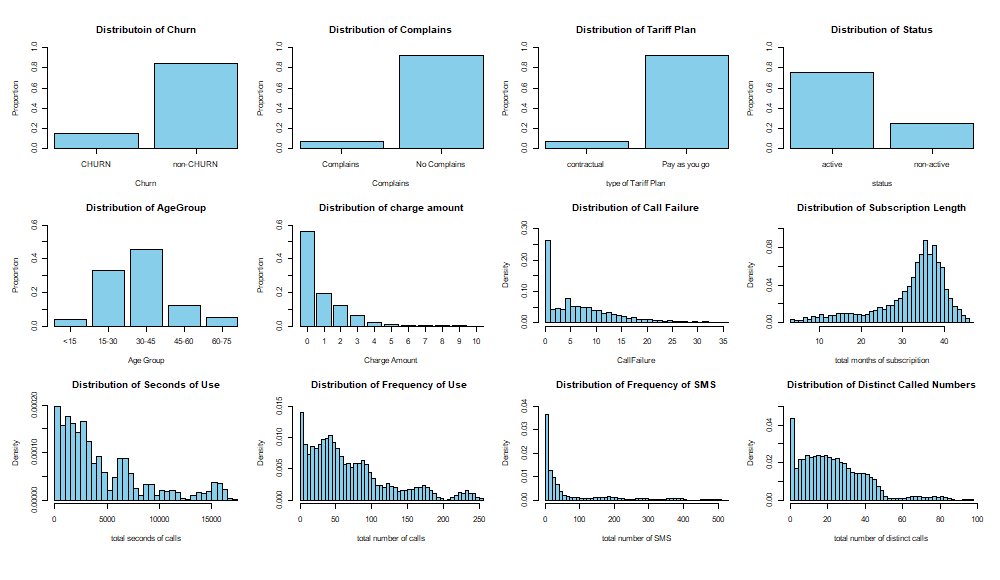
\includegraphics[width=1\linewidth]{univariate_analysis.png}
    \caption{Univariate Plot of the variables.}
    \label{fig:univariate}
\end{figure}

\subsection{Bivariate Analysis - correlations between variables}

Now instead of investigating single variables, we explore the relationships between two variables. The two important bivariate analysis topics are 1) the relationship between outcomes and the covariates, and 2) the correlations in-between the covariates. 

Below is a very informative plot demonstrating the most relevant information in all continuous variables and the outcome Churn. 

\begin{figure}[H]
    \centering
    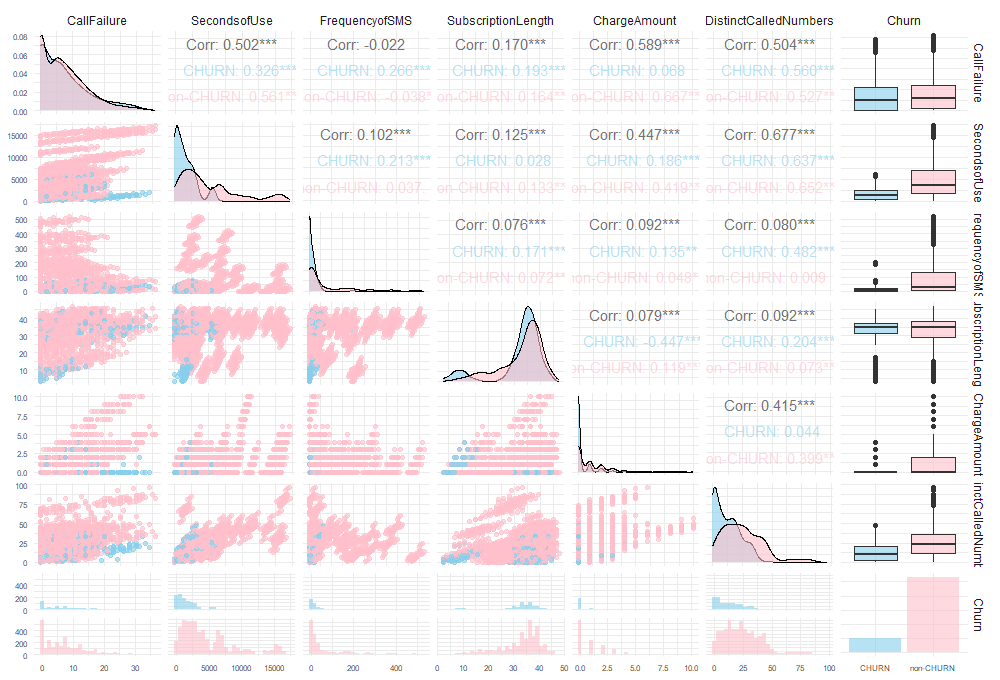
\includegraphics[width=1\linewidth]{pairs_plot.png}
    \caption{Paris plot of all continuous variables and the outcome Churn}
    \label{fig:pairsplot}
\end{figure}

Most features show a different distribution with respect to different customer churning behaviour. For example,  in the case of total frequency/seconds of calls, observe that customers who churned (blue) demonstrate a clearly lower usage of calling services compared to non-churn customers (pink). 

Also, notice how the company indeed received more complaints in the churned group, who also use the the "pay as you go" plan instead of subscriptions. This agrees with common sense as it indicates a lower brand loyalty. 

\textbf{Multicollinearity}

Notice also that the multicollinearity problem exists in our dataset. Figure \ref{fig:multicolin} gives the pairwise correlation information of all continuous variables in the dataset. All pairs of covariates exhibit a positively correlated relationship to some extent. 

\begin{figure}
    \centering
    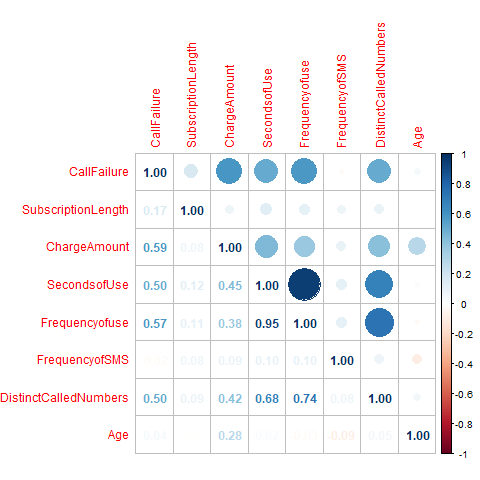
\includegraphics[width=0.6\linewidth]{multicollinearity.png}
    \caption{Multicollinearity heatmap of all continuous covariates}
    \label{fig:multicolin}
\end{figure}

Specifically, it is very clear that the frequency of use and the second of use gives a correlation almost equal to one. This is not a surprise as they basically predict the same thing. If both variables are included in the model, then we may need to pay close attention to the independence assumption of the (generalised) linear model which is very likely violated. 

Additionally, the subscription length is uncorrelated with most other (continuous) variables. 

\subsection{Transformation - linearity assumption for GLMs}

The following initial empirical logit plots shows that most of the relationships between the link and the variables are non-linear, e.g., months of subscription, seconds/frequency of calls/SMSs etc. This violates the linearity assumption and hence needed to be transformed before fitting into the GLM model. 

\begin{figure}[H]
    \centering
    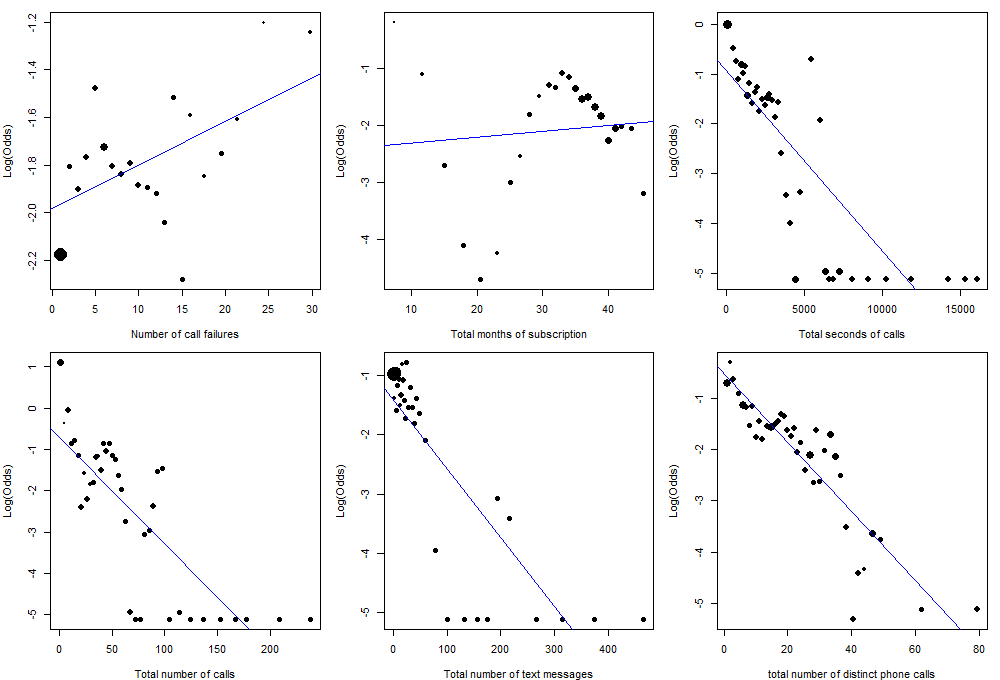
\includegraphics[width=1\linewidth]{emplogit_init.png}
    \caption{Initial Empirical Logit plots}
    \label{fig:enter-label}
\end{figure}

Notice that the months of subscription variable clearly shows a cubic relationship with the links, \
(logit($\mathbb{P}($Churn$)$), which indicates that a cubic polynomial term might be needed for a logistic regression model. 

Therefore, we tried several different transformation methods, including square-root transformation, log transformation and the inverse transformation, and the transformed empirical logit plot, Figure \ref{fig:emplogit} indicated the relationship between the square-root transformed variable and the logit link is the most linear with the least violation of the linearity assumption. 

In conclusion, we flagged that the \texttt{Seconds of Use}, \texttt{Frequency of use}, and \texttt{Frequency of SMS} variables need to be square-root transformed before logistic modelling. 

\begin{figure}[H]
    \centering
    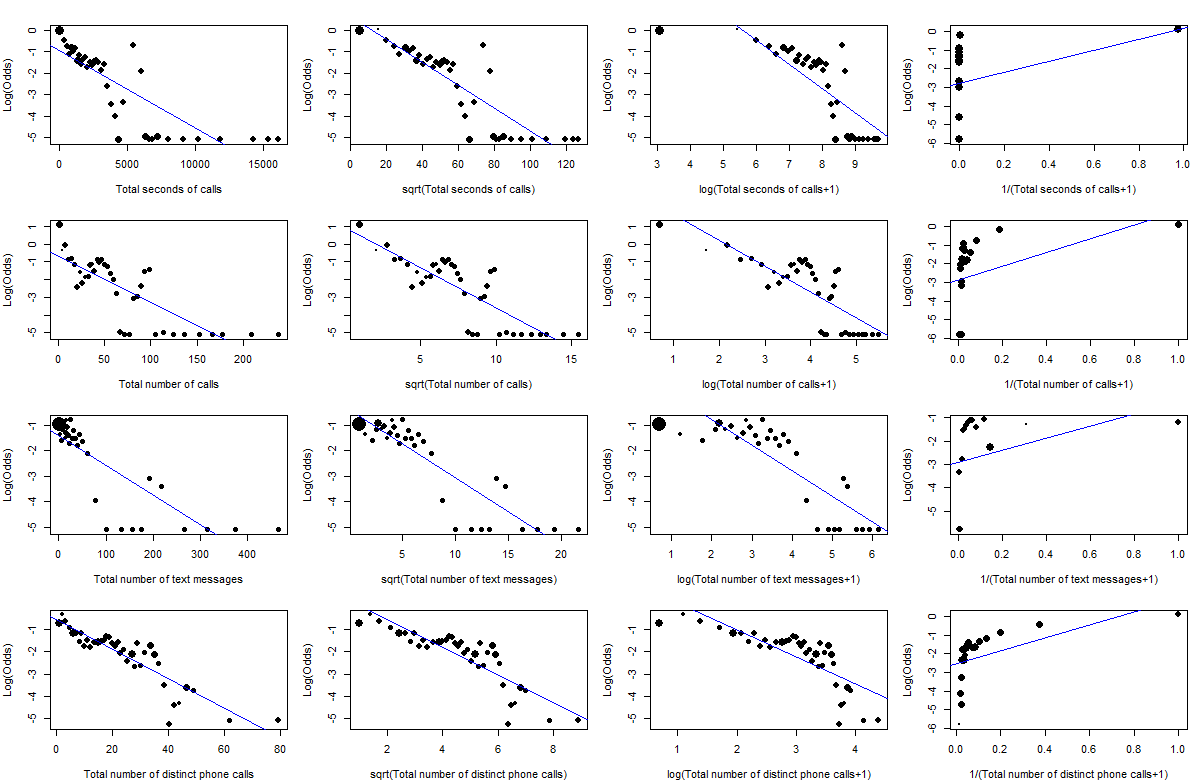
\includegraphics[width=1\linewidth]{emplogit.png}
    \caption{Empirical logit plot for continuous variables}
    \label{fig:emplogit}
\end{figure}

Notice that standardisation is needed in some models (discussed later in Section \ref{sec:modelling}), we also plot the empirical logit plot after transformation and then standardisation in Figure \ref{fig:emplogitscaled}. 

\begin{figure}[h]
    \centering
    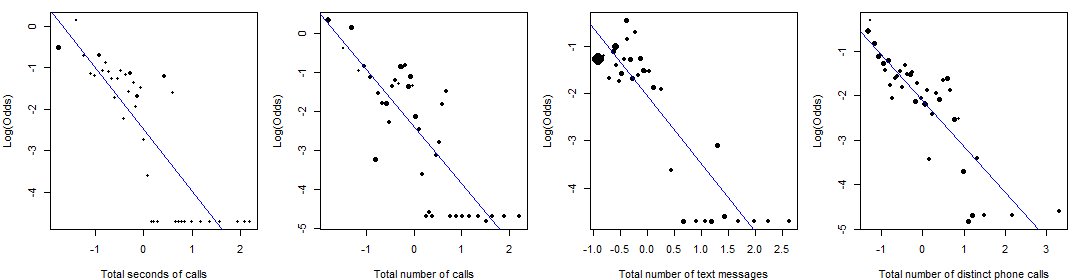
\includegraphics[width=1\linewidth]{emplogit_scaled.png}
    \caption{Empirical Logit plot of variables after transformation and standardisation (left 1-3 figures), or standardisation only (rightmost)}
    \label{fig:emplogitscaled}
\end{figure}


\subsection{Train-test Split Check}

\begin{figure}[H]
    \centering
    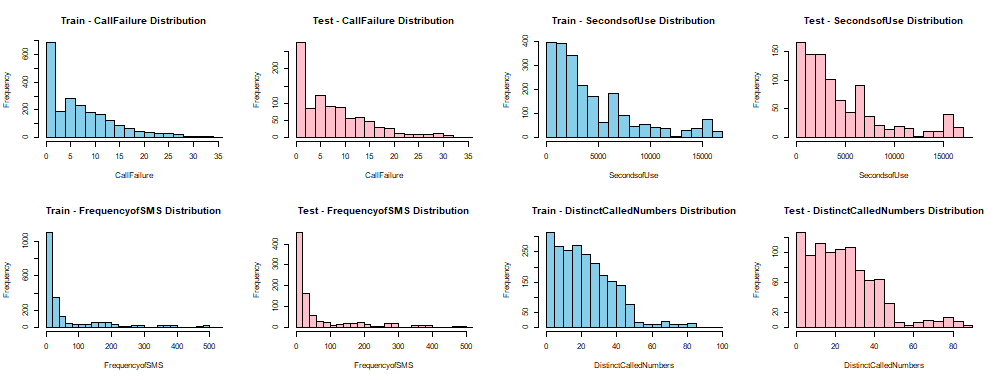
\includegraphics[width=1\linewidth]{mimic_checks_continuous.png}
    \caption{Checking test dataset mimics the training dataset for discrete variables}
    \label{fig:mimicscont}
\end{figure}

One more thing we need to check in the EDA section is that the test set mimics the patterns and distributions of the training dataset. This is to ensure that our model performance check on the test set is valid, representative, and generalisable. Figure \ref{fig:mimicscont}, and Figure \ref{fig:mimcsdisc} shows that the univariate distribution of the variables are correctly represented in the test set. 

\begin{figure}[h]
    \centering
    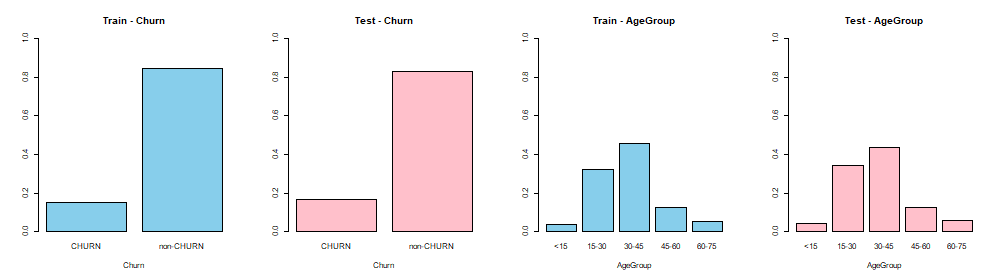
\includegraphics[width=1\linewidth]{mimic_checks_discrete.png}
    \caption{Checking test dataset mimics the training dataset for discrete variables}
    \label{fig:mimcsdisc}
\end{figure}

\section{Model Fitting}\label{sec:modelling}

After careful consideration, in this report we will implement and test for 4 models, they are: 

\begin{enumerate}
    \item AIC stepwise selected model
    \item BIC stepwise selected model
    \item LASSO penalised regression model
    \item Support Vector Machine (SVM) model with kernel trick
\end{enumerate}

Notice that, in this section, we use the training set only. As described in the EDA Section \ref{sec:EDA}, 3 variables are pre-transformed using square-root transformation for \textbf{model 1, 2, and 3}, and then all continuous variables are then standardised to mean 0 with standard deviation 1 for \textbf{model 3}. The \textbf{model 4} use the dataset with standardisation procedure without transformation.  

\subsection{Initial Full model}

With adjusted for all transformations, polynomial terms, and including all available features in our model, we now obtain the initial full logistic regression model as below: 

$$
\begin{aligned}
\text{logit}(\mathbb{P}(\text{Churn})) = \beta_0 
&+ \beta_1 {\texttt{CallFailure}} 
+ \beta_2 \mathbf{1}_{\texttt{Complains=yes}} 
+ \beta_3 {\texttt{SubscriptionLength}}\\
&
+ \beta_4 {\texttt{SubscriptionLength}^2}
+ \beta_5 {\texttt{SubscriptionLength}^3} 
+ \beta_6 {\texttt{ChargeAmount}} \\
& + \beta_7 \mathbf{1}_{\texttt{Age in 15-30}} 
+ \beta_8 \mathbf{1}_{\texttt{Age in 30-45}} 
+ \beta_9 \mathbf{1}_{\texttt{Age in 45-60}} 
+ \beta_{10} \mathbf{1}_{\texttt{Age in 60-75}} \\
& + \beta_{11} \mathbf{1}_{\texttt{TariffPlan=contractual}} 
+ \beta_{12} \mathbf{1}_{\texttt{Status=non-active}} \\
&+ \beta_{13} \texttt{Distinct Called Numbers}
+ \beta_{14} \sqrt{\texttt{Second of Use}} \\
&+ \beta_{15} \sqrt{\texttt{Frequency of use}}
+ \beta_{16} \sqrt{\texttt{Frequency of SMS}}
\end{aligned}
$$

\subsection{Stepwise Selection}

Stepwise selection involves iterative processes to either add or drop variables based on information criteria like AIC or BIC. Our stepwise selection alternates between forward and backward direction (\texttt{direction = both}) to move toward the model which improves the criterion the most, and stopped until AIC/BIC could not be improved by adding to dropping variables any further. 

\subsection{Grouped Lasso Method}

Just like Lasso variable selection method, one more step that the \texttt{gglasso} method allows us to select multiple parameters together, i.e. either select the group of parameters together or send all parameters in the group to exactly 0. This allows us to perform variable selection via L1 norm penalised regression modelling for original categorical variables. 

As a convention, we use the $\lambda$ (penalise parameter) which gives Mean Square Error (MSE) within 1 standard deviation of the minimum MSE (right dotted line Figure \ref{gglassocv}). This is to prevent overfitting and give a more parsimonious model within a reasonable range. 

\begin{figure}[H]
    \centering
    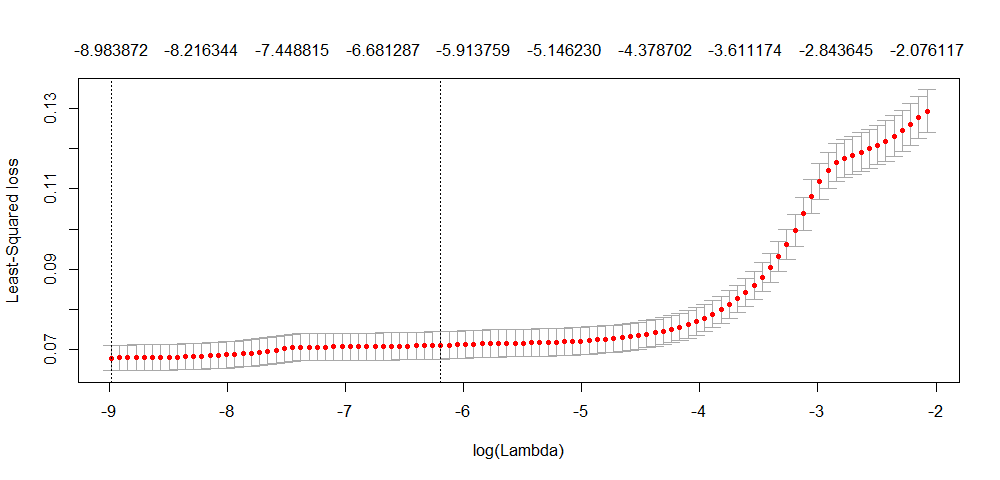
\includegraphics[width=1\linewidth]{gglasso_cv.png}
    \caption{Cross-validation result for Grouped Lasso method.}
    \label{fig:gglassocv}
\end{figure}


\subsection{Support vector machine}

The strengths of the Support Vector Machine (SVM) include its effectiveness in high-dimensional spaces and versatility in handling various types of data and relationships (e.g., non-linear) by the kernel tricks. Hence it is particularly suitable for the binary classification task in our case, as our data has several non-linearity problems as discussed in the transformation section. 

SVM operates by finding the hyperplane that optimally separates different classes in the feature space. It maximizes the margin between the nearest data points of any class (known as support vectors). 

Notice also, in this modelling process, we do not transform the variables, but only standardise the continuous feature variables since SVM is also sensitive to scale due to the notion of maximum margin. 

\subsection{Vairable Selection Summary} 

After implemented the above models, the summary of variable selection results are as below: 

\begin{table}[h]
    \centering
    \begin{tabular}{|@{}l|llll|@{}}
    \toprule
    \textbf{Variable} & \textbf{AIC} & \textbf{BIC}  & \textbf{gglasso} & \textbf{SVM} \\ 
    \midrule
    Call Failure & \checkmark & \checkmark & \checkmark & \checkmark \\
    Complains & \checkmark& \checkmark& \checkmark& \checkmark \\
    I(Subscription Length)^3 & \checkmark & \checkmark &  & \checkmark \\
    Charge Amount & \checkmark & \checkmark & \checkmark & \checkmark \\
    Seconds of Use & &  & \checkmark & \checkmark \\
    Frequency of use & \checkmark & \checkmark & \checkmark & \checkmark \\
    Frequency of SMS & \checkmark & \checkmark & \checkmark & \checkmark \\
    Distinct Called Numbers &  & \checkmark &  & \checkmark \\
    Age Group  & \checkmark &  &  & \checkmark \\
    Tariff Plan &  &  &  & \checkmark \\
    Status & \checkmark & \checkmark & \checkmark & \checkmark \\
    \bottomrule
    \end{tabular}
    \caption{Summary of Outcome and Feature variables in the Dataset}
    \label{table:varselection}
\end{table}

We noticed that the \texttt{gglasso} select the least number of variables, and the SVM model does not perform variable selection hence all variables are selected. 

Also, some variables are selected by all variable selection process, they are: Call Failure, Complains, Charge Amount, Frequency of use, Frequency of SMS and Status. 

\section{Model Evaluation}

\subsection{Model Performance}

Now, in this section, we use the test set only. 

Our primary goal is to examine the performance of the models. Hence to do so, we follow the following steps: 

\begin{enumerate}
    \item predict the fitted response, i.e. the probability of Churn, by using the trained models 1 to 4 based on the feature variables in the test set
    \item assign the customer to Churn group if the probability of churning is > 0.5, and to non-Churn group is <=0.5
    \item produce the confusion matrix of the models and calculate the accuracy of the prediction. 
    \item plot the ROC curve of the binary classification model, and calculate the corresponding AUC. 
\end{enumerate}

Given the 0.5 threshold, the 4 confusion matrix is given by: 

\

\

\textbf{AIC model: }

$$
\begin{array}{cc|c|c|}
& \multicolumn{1}{c}{} & \multicolumn{2}{c}{\text{True Label}} \\
& \multicolumn{1}{c}{} & \multicolumn{1}{c}{\text{non-Churn}} & \multicolumn{1}{c}{\text{Churn}} \\ \cline{3-4}
\multirow{2}{*}{\text{Prediction}} & \text{non-Churn} & 770 & 69 \\ \cline{3-4}
& \text{Churn} & 16 & 90 \\ \cline{3-4}
\end{array}
$$

Accuracy: 91.01\%
Sensitivity: 97.96\%    
Specificity: 56.60\% 

\textbf{BIC model: }

$$
\begin{array}{cc|c|c|}
& \multicolumn{1}{c}{} & \multicolumn{2}{c}{\text{True Label}} \\
& \multicolumn{1}{c}{} & \multicolumn{1}{c}{\text{non-Churn}} & \multicolumn{1}{c}{\text{Churn}} \\ \cline{3-4}
\multirow{2}{*}{\text{Prediction}} & \text{non-Churn} & 776 & 74 \\ \cline{3-4}
& \text{Churn} & 10 & 85 \\ \cline{3-4} 
\end{array}
$$

Accuracy: 91.11\%
Sensitivity: 98.73\%          
Specificity: 53.46\% 

\textbf{gglasso model:}

$$
\begin{array}{cc|c|c|}
& \multicolumn{1}{c}{} & \multicolumn{2}{c}{\text{True Label}} \\
& \multicolumn{1}{c}{} & \multicolumn{1}{c}{\text{non-Churn}} & \multicolumn{1}{c}{\text{Churn}} \\ \cline{3-4}
\multirow{2}{*}{\text{Prediction}} & \text{non-Churn} & 776 & 104 \\ \cline{3-4}
& \text{Churn} & 10 & 55 \\ \cline{3-4} 
\end{array}
$$

Accuracy: 87.94\%
Sensitivity: 98.73\%         
Specificity: 34.59\%

\textbf{SVM model: }

$$
\begin{array}{cc|c|c|}
& \multicolumn{1}{c}{} & \multicolumn{2}{c}{\text{True Label}} \\
& \multicolumn{1}{c}{} & \multicolumn{1}{c}{\text{non-Churn}} & \multicolumn{1}{c}{\text{Churn}} \\ \cline{3-4}
\multirow{2}{*}{\text{Prediction}} & \text{non-Churn} & 782 & 104 \\ \cline{3-4}
& \text{Churn} & 4 & 55 \\ \cline{3-4} 
\end{array}
$$

Accuracy: 88.57\%,
Sensitivity: 99.49\%,    
Specificity: 34.59\%

\textbf{summary on confusion matrices: }

The highest accuracy is given by the BIC model, 91.11\% accuracy. 

The \texttt{gglasso} model and the SVM model gives a higher sensitivity but lower specificity compared to the stepwise selected model using a 0.5 probability threshold. However, considering the high cost of NOT applying any retention strategy to the churning customers, a higher specificity is normally considered more important than a minor improvement in sensitivity. 

Hence, in the analysis of model performance metrics, the BIC model gives the best performance due to its high accuracy and high specificity. 


\textbf{ROC and AUC analysis}

In addition, we may want to the ROC plots of the 4 models are given in Figure \ref{fig:roc}. Clearly, the SVM model gives the best roc with the highest area-under-curve (AUC) value. 

\begin{figure}[h]
    \centering
    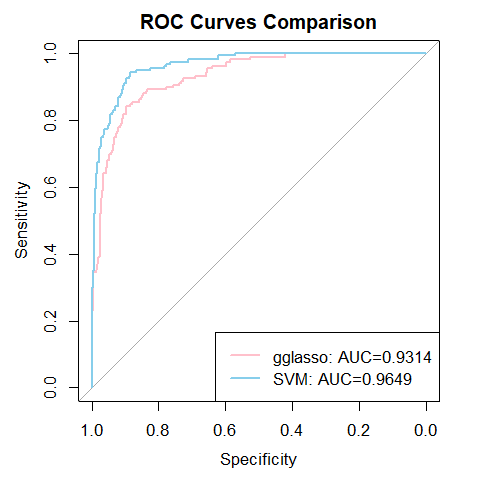
\includegraphics[width=0.6\linewidth]{roc.png}
    \caption{The ROC plots for all 4 models}
    \label{fig:roc}
\end{figure}


We notice that, actually in the specificity Vs sensitivity analysis, the model performs both higher sensitivity and higher specificity is the SVM model. Improving both values can be done by moving the classification threshold. 

\subsection{Model Diagnostics}

To confirm that the BIC model is indeed a good fit for the dataset, we also need to make sure that the model meet the assumptions well. Below is the diagnostics plots for the BIC model, and we may conclude from the following plots that the model assumptions are properly met, since: 

\begin{itemize}
    \item Cook's distances are all very small ($<$ 0.05). 
    \item The influence plot seems to have no outliers with high leverages. 
    \item all points fall in the confidence interval of the half-normal plot and it shows a reasonable linear relationship. 
\end{itemize}

\begin{figure}[h]
    \centering
    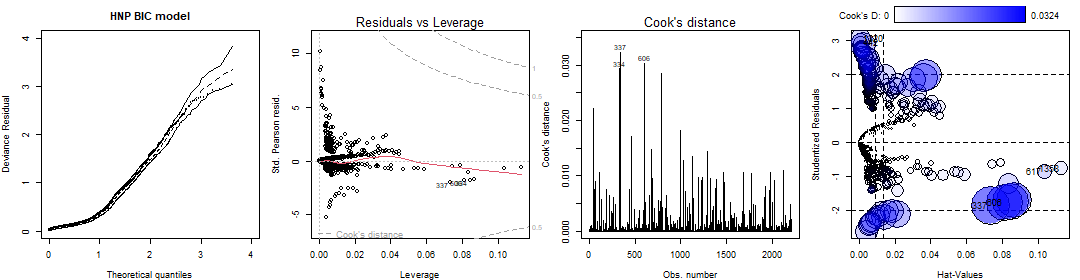
\includegraphics[width=1\linewidth]{stepwiseBIC_diagnostics.png}
    \caption{Model Diagnostics plots for the Stepwise BIC model. }
    \label{fig:BICdiagnostics}
\end{figure}

\section{Conclusion and interpretations} 

Both the SVM model and the BIC model give high performance, however the SVM model gives a better ROC with different decision thresholds. This is not part of our analysis in this report. 

Therefore, based on all analyses before, we chose the BIC model as our final model, below is the final model formula and the coefficients. 

$$
\begin{aligned}
\text{logit}(\mathbb{P}(\text{Churn})) = \beta_0 
&+ \beta_1 {\texttt{CallFailure}} 
+ \beta_2 \mathbf{1}_{\texttt{Complains=yes}} 
+ \beta_3 {\texttt{SubscriptionLength}}\\
&
+ \beta_4 {\texttt{SubscriptionLength}^2}
+ \beta_5 {\texttt{SubscriptionLength}^3} 
+ \beta_6 {\texttt{ChargeAmount}} \\
& + \beta_7 \mathbf{1}_{\texttt{Status=non-active}} 
+ \beta_8 \sqrt{\texttt{Frequency of use}}
+ \beta_9 \sqrt{\texttt{Frequency of SMS}}
\end{aligned}
$$

\begin{table}[h]
\centering
\caption{Model Estimates}
\begin{tabular}{lr}
\toprule
\textbf{Variable} & \textbf{Estimate} \\
\midrule
(Intercept) & 0.02549 \\
Call Failure & 1.12131 \\
Complains: No Complains & -3.91967 \\
poly(Subscription Length, 3) 1 & -6.34295 \\
poly(Subscription Length, 3) 2 & 14.93371 \\
poly(Subscription Length, 3) 3 & -26.90285 \\
Charge Amount & -0.66984 \\
Status: non-active & 1.20880 \\
Frequency of Use & -1.39272 \\
Frequency of SMS & -0.80167 \\
\bottomrule
\end{tabular}
\end{table}

Example interpretation: 

\textbf{Call Failure: }

For each additional call failure, the log odds of churning increase by 1.12131. This suggests that customers experiencing more call failures are significantly more likely to churn, reflecting a strong positive relationship between call failures and customer churn.

\textbf{Charge Amount: }

This coefficient indicates that as the charge amount increases (within its ordinal levels from 0 to 9), the log odds of churning decrease by 0.66984. Higher charges, possibly indicating higher usage or more premium services, appear to reduce the likelihood of churn.

\section{Further Discussions}

Misclassification cost is a big problem, due to the different losses if we do not apply retention strategy to churning groups or if we apply retention churning strategy to the non-churn group. 

People may want to try neural network models or bayesian modelling techniques to the dataset to improve the accuracy, but due to time constraints, these methods are not included in this report. 

\newpage

\section*{Reference}

Jafari-Marandi, R., Denton, J., Idris, A., Smith, B. K., & Keramati, A. (2020). Optimum profit-driven churn decision making: innovative artificial neural networks in telecom industry. Neural Computing and Applications, 32, 14929-14962. 

Y. Yang (2024). Group Lasso Penalized Learning Using a Unified BMD Algorithm. 

M. Huang, T Brunsdon (2023). Applied Statistics Modelling Modules: Iranian Churn Data Analysis, University of Warwick. 

\end{document}                                                    
                                                                           
                                                                           
                                                                           
                                                                           
                                                                           
                                                                           
                                                                           
                                                            